\documentclass[12pt]{article}
\usepackage[a4paper, left=3cm, right=3cm]{geometry}	% Per i margini
\usepackage[latin1]{inputenc}
\usepackage{amssymb}
\usepackage{color, xcolor}
\usepackage{graphicx}	% Per immagini e pdf.
\usepackage{amsmath}

\title{Progetto di Sistemi per il Governo dei Robot mod. A}
\author{Riccardo Grieco, Marco Matarese, Andrea Pollastro}

\begin{document}
	%\maketitle
	% --- TITLE PAGE --- %

\thispagestyle{empty}

\begin{center}
	
\includegraphics[width=0.8\textwidth]{images/DIETI}\\
	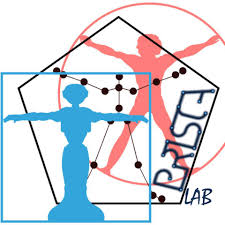
\includegraphics[width=0.2\textwidth]{images/prisca.jpg}
	
	\par\bigskip\par\bigskip\par\bigskip
	%\par\bigskip\par\bigskip\par\bigskip\par\bigskip\par\bigskip\par\bigskip\par\bigskip\par	% Per spazi
	
	{\huge Touch the Color\\}
	%{\huge Algoritmi e Strutture Dati II\\}
	
	\par\bigskip\par\bigskip\par\bigskip\par\bigskip\par\bigskip\par\bigskip\par\bigskip\par	% Per spazi
	
	{\LARGE Progetto di \\}
	{\LARGE Sistemi per il Governo dei Robot mod. A\\}
	{\large A.A 2018/2019\par}
	
	\par\bigskip\par\bigskip\par\bigskip\par\bigskip\par\bigskip\par\bigskip
	
	{\large Grieco Riccardo N97/28 \\}
	{\large Matarese Marco N97/280 \\}
	{\large Pollastro Andrea N97/28 \\}
	
	\par\bigskip\par\bigskip\par\bigskip\par\bigskip\par\bigskip\par\bigskip	
	
	
	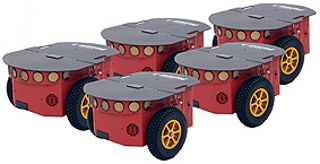
\includegraphics[width=0.3\textwidth]{images/pioneer.jpg}
\end{center}

	\newpage
	
	\tableofcontents
	
	\newpage
	
	\section{Introduzione}	% descrizione del progetto
		% nicchia ecologica: ambiente, robot, robe...
		% descrizione del gioco: ruoli, interazione, scopo.
		% schema dei behaviour
		\newpage
		
	\section{Modulo Motorio}
		% campi di potenziale
		% descrizione wander
		% descrizione avoid
		% descrizione move to color
		% descrizione sussunzioni
		\newpage
		
	\section{Modulo per la Comunicazione}
		% socket
		% protocollo di comunicazione
		\newpage
		
	\section{Modulo di Visione}
		% openni e kinect
		% conversione RGB to HSV
		% ricerca dei blob e del centroide
		% uso della profondit�
		\newpage
	
	\section{Esperimenti}
		% cazzo ne so...
		\newpage
	
\end{document}